\documentclass{article} % For LaTeX2e
\usepackage{nips12submit_e,times}
 \nipsfinalcopy % Uncomment for camera-ready version
\usepackage{graphicx}
\usepackage{amsmath}
\usepackage{amssymb}
\usepackage{amsthm}
\usepackage{hyperref}
\usepackage{graphicx}

\newcommand{\B}[1]{{\bf #1}}
\newcommand{\Sc}[1]{{\mathcal{#1}}}
\newcommand{\R}[1]{{\rm #1}}
\newcommand{\mB}[1]{{\mathbb{#1}}}
%%%%%%%%%%%%%%%%%%%%%%%%%
% Commands copied from hart.sty
\newcommand{\bB}{\bf{B}}\newcommand{\bN}{\bf{N}}
% \newcommand{\B{1}}{\mathbb {1}}
%%%%%%%%%%%%%%%%%%%%%%%%%


% Macros added by Burke
\newcommand{\set}[2]{\left\{#1\,\left\vert\, #2\right.\right\}}
\newcommand{\one}{\bf{1}}
\newcommand{\half}{\frac{1}{2}}
\newcommand{\map}[3]{#1\,:\,#2\rightarrow #3}
\newcommand{\cS}{\mathcal{S}}
\newcommand{\cL}{\mathcal{L}}




\newtheorem{lemma}{Lemma}[section]
%\newtheorem{remark}{Remark}[section]
\newtheorem{remark}[lemma]{Remark}
\newtheorem{theorem}[lemma]{Theorem}
\newtheorem{corollary}[lemma]{Corollary}
\newtheorem{conjecture}[lemma]{Conjecture}
\newtheorem{proposition}[lemma]{Proposition}
\newtheorem{definition}[lemma]{Definition}
\newtheorem{algorithm}[lemma]{A}

\title{Predict Energy Consumption with Deep Learning Models using Weather Data}


\author{
John Min\\
Departments of Operating Research\\
Columbia Unniversity, New  York\\
\texttt{jcm2199@columbia.edu} \\
\And
Victor Ferrand\\
Department of Computer Science \\
Columbia University, New York\\
\texttt{vf2221@columbia.edu} 
}

% The \author macro works with any number of authors. There are two commands
% used to separate the names and addresses of multiple authors: \And and \AND.
%
% Using \And between authors leaves it to \LaTeX{} to determine where to break
% the lines. Using \AND forces a linebreak at that point. So, if \LaTeX{}
% puts 3 of 4 authors names on the first line, and the last on the second
% line, try using \AND instead of \And before the third author name.

\newcommand{\fix}{\marginpar{FIX}}
\newcommand{\new}{\marginpar{NEW}}

%\nipsfinalcopy % Uncomment for camera-ready version

\begin{document}


\maketitle

\begin{abstract}
Demand load forecasting is an integral component of optimizing energy consumption. For energy providers, excess demand causes "brownouts" while excess supply wastes fuel and augments the carbon footprint of the provider. The problem is analogous for building engineeers who everyday face the trade-off between the high cost of energy versus insufficient consumption which could result in uncomfortable building temperatures. Predicting a building's steam demand using weather and building temperature variables is a non-trivial, non-linear problem -- the underlying structure of these interactions is not well-known and suggests the need for a complex model.  Thus, we turn to neural networks and deep learning algorithms such as Restricted Boltzmann Machines (RBMs) to construct Deep Belief Networks (DBNs) and compare the results to that of other machine learning algorithms and time series modeling methodology. 

\end{abstract}

\vspace{-.2cm}
\section{Introduction}
\vspace{-.2cm}

\begin{Introduction}
A crucial part of optimizing energy consumption is demand load forecasting, the ability to recognize patterns of consumption. Energy providers are wary of excess demand which causes "brownouts" and of excess supply which squanders and misuses valuable fuel. Building engineers face an analogous problem in optimizing energy consumption by balancing building comfort and demand with the high cost of usage. Using weather prediction variables and real-time building temperatures by quadrant, we predict building steam consumption throughout the day. The underlying structure behind steam usage is a non-linear, non-trivial problem that has yet to be solved.\\

\noindent
The building data comes from a large commercial building in Manhattan where the building management system (BMS) is tracking and storing real-time building temperatures and energy consumption every 15 minutes. Weather data comes from Weather Underground, a commercial weather service, or from the National Oceanic and Atmospheric Administration (NOAA), both having APIs that enable access to hourly weather observation and forecast data. The weather covariates are linearly interpolated to align the building data with the weather data (which generally is produced on the 51st or 52nd minute of the hour). In addition to building temperature data, the other variables include temperature, dewpoint, humidity, humidex, windspeed, luminosity, pressure, windchill, heat index, precipitation (binary), the day of week (categorical), and federal holiday (binary). Seemingly reasonable to assume that past steam usage affecfts future consumption, Markov lags on steam are also considered.
\\

\noindent
Time-series modeling of steam consumption has not been straightforward because the model must capture the daily periodicity, seasonality, and non-linear nature of the underlying structure. As we show in the next section, models such as linear regression, support vector regression, which kernelizes the inputs into a higher-dimensional space using a Gaussian kernel, and random forest regression, which in the literature has demonstrated strong empirical regression results, all fail to capture the complexity of the steam process. Part of the problem may be that the behavior of the building engineers in operating the BMS is not consistent. However, the goal for these engineers has never changed: keep the building temperature between 70 and 75 degrees Fahrenheit during business hours. If a quadrant in the building appears to be cooler than the lease requirement, it is expected that hot air (using steam) will be pumped through the Heating, Ventilation, and Air Conditioning (HVAC) sytem. Analogously, if the building is hot in the summer, steam-powered chillers would be used to cool down the building. \\

\noindent
Weather is the primary driver of thermodynamic change in the building. To combat the effects that weather has on building temperature, the engineers use steam to enact change to respond to how the building is behaving. It is not our belief that the data is insufficient in being to recognize patterns with the steam consumption process. Rather, we believe model complexity is the key to improving our predictions. Instead of spending a lot of time on developing and testing numerous kernels, we turn to the power of neural networks and deep learning algorithms such as Restricted Boltzmann Machines (RBMs) to construct Deep Belief Netweorks (DBNs) that encode and represent the data in a space that may more effectively capture the complex structure of the data.
\end{Introduction}


%%%%%%%%%%%%%%%%%%%%%%%%%%%%%%%%%%%%%%%%%%%%%%%%%%%%%%%%%%%%%%%%%%%%%%%%%%
% Classical Methods
%%%%%%%%%%%%%%%%%%%%%%%%%%%%%%%%%%%%%%%%%%%%%%%%%%%%%%%%%%%%%%%%%%%%%%%%%% 

\vspace{-.2cm}
\section{Simple Models}
\vspace{-.2cm}

The simple models, encompassing linear regressions, support vector machine, random forest, etc, do a poor even miserable job on steam demand prediction. With a relative error from 200$\%$  to 300$\%$ these models obviously do not fit the underlying structure of weather/energy interactions. 
\\We ran some of the classical regression models on our data to be convinced of this assertion, and our expectation were more than confirmed. Randomly predicted values would have nearly done the same work ! We plotted the absolute errors in thousands of pounds per hour across the whole 2012 year.
\\
\\Plots:

\begin{center}
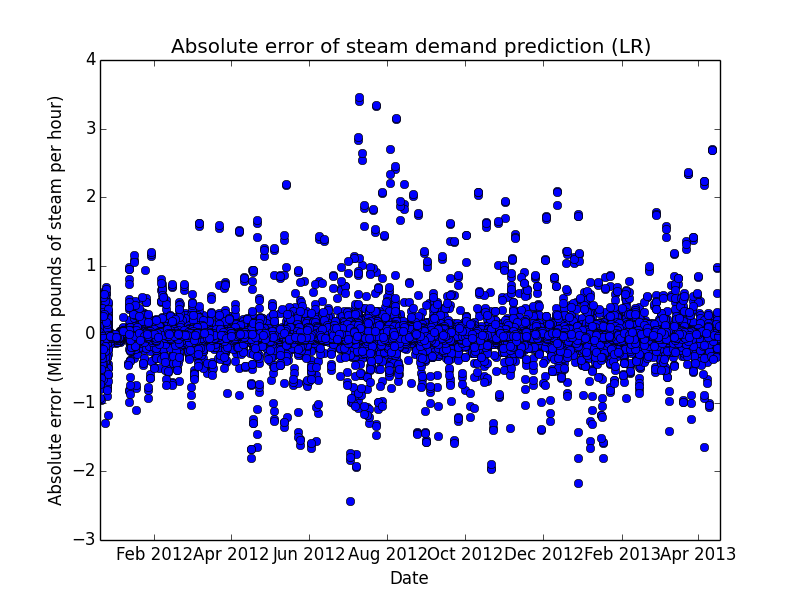
\includegraphics{LR_error}[scale=0.1]
\end{center}

\begin{center}
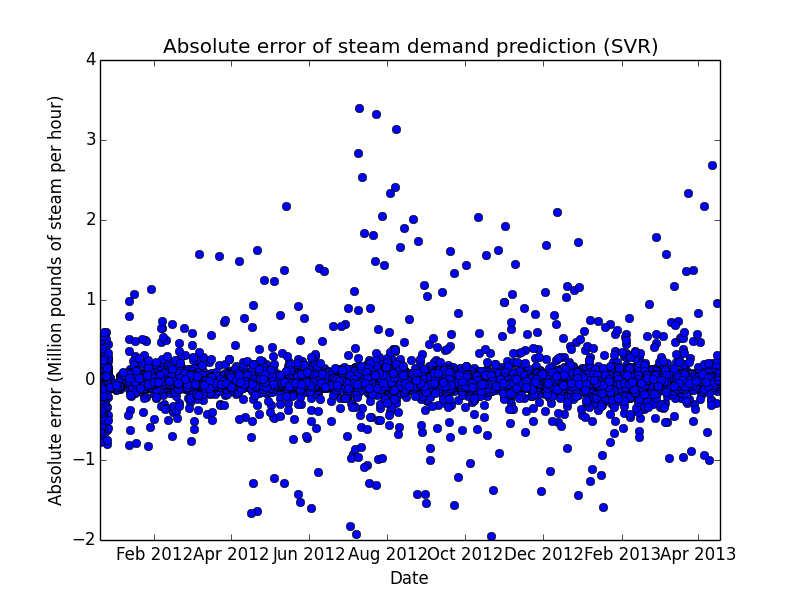
\includegraphics{SVR_error}[scale=0.1]
\end{center}
%%%%%%%%%%%%%%%%%%%%%%%%%%%%%%%%%%%%%%%%%%%%%%%%%%%%%%%%%%%%%%%%%%%%%%%%%%
% Implementation NN RBM DBN
%%%%%%%%%%%%%%%%%%%%%%%%%%%%%%%%%%%%%%%%%%%%%%%%%%%%%%%%%%%%%%%%%%%%%%%%%% 


\vspace{-.2cm}
\section{Implementation of Neural Networks, Restricted Boltzmann's Machine and Deep Belief Networks}
\vspace{-.2cm}

\subsection{Neural Networks}

\subsection{Restricted Boltzmann Machine}

\subsection{Deep Belief Networks}


%%%%%%%%%%%%%%%%%%%%%%%%%%%%%%%%%%%%%%%%%%%%%%%%%%%%%%%%%%%%%%%%%%%%%%%%%%
% Deep Learning Results 
%%%%%%%%%%%%%%%%%%%%%%%%%%%%%%%%%%%%%%%%%%%%%%%%%%%%%%%%%%%%%%%%%%%%%%%%%% 


\vspace{-.2cm}
\section{Numerical Results and Plots}
\vspace{-.2cm}



%%%%%%%%%%%%%%%%%%%%%%%%%%%%%%%%%%%%%%%%%%%%%%%%%%%%%%%%%%%%%%%%%%%%%%%%%%
% Conclusions
%%%%%%%%%%%%%%%%%%%%%%%%%%%%%%%%%%%%%%%%%%%%%%%%%%%%%%%%%%%%%%%%%%%%%%%%%% 


\vspace{-.2cm}
\section{Conclusion}
\vspace{-.2cm}


\newpage
\section{Bibliography}
\bibliographystyle{plain}
%\bibliography{filter}



\newpage
\section{Appendix}




\end{document}
